% 78-44(78쪽) — 호 AB 를 10등분한 사분원(원문 「오른쪽 그림」). 스캔 화질이 낮아 TikZ 로 다시 그림.
% 라벨은 원문 것만: $\pt{O}$·$\pt{A}$·$\pt{B}$ 와 등분점 $\pt{A_1}$·$\pt{A_2}$·$\pt{A_9}$, 각 $\theta$.
% 원문처럼 반지름은 $\seg{OA_1}$·$\seg{OA_2}$·$\seg{OA_9}$ 만 긋고 가운데 생략 부분은 점 세 개로 둔다.
% 반지름 길이·각의 크기 눈금은 원문에 없으므로 적지 않는다(답이 그림에서 읽히지 않게).
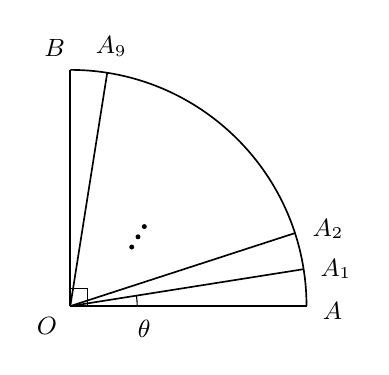
\begin{tikzpicture}[line width=0.6pt, x=1cm, y=1cm]
  \draw (3,0) arc (0:90:3);
  \draw (0,0) -- (3,0);
  \draw (0,0) -- (0,3);
  \draw (0,0) -- (2.963,0.469);
  \draw (0,0) -- (2.853,0.927);
  \draw (0,0) -- (0.469,2.963);
  \draw[line width=0.45pt] (0.22,0) -- (0.22,0.22) -- (0,0.22);
  \draw[line width=0.4pt] (0.85,0) arc (0:9:0.85);
  \fill (0.78,0.75) circle (0.9pt);
  \fill (0.86,0.88) circle (0.9pt);
  \fill (0.94,1.01) circle (0.9pt);
  \node[font=\small, anchor=north east] at (-0.04,-0.02) {$\pt{O}$};
  \node[font=\small, anchor=west] at (3.08,-0.06) {$\pt{A}$};
  \node[font=\small, anchor=west] at (3.05,0.47) {$\pt{A_1}$};
  \node[font=\small, anchor=west] at (2.95,0.98) {$\pt{A_2}$};
  \node[font=\small, anchor=south] at (0.52,3.04) {$\pt{A_9}$};
  \node[font=\small, anchor=south east] at (0.06,3.04) {$\pt{B}$};
  \node[font=\small, anchor=north] at (0.94,-0.05) {$\theta$};
\end{tikzpicture}
